\section*{2010}
\vspace{-.5cm}
\hrulefill \smallskip\\
\ques{1}{c}{12} What is rectifying inspection plan? Obtain the expressions for AOQ and ATI, with reference to a single sampling plan for attributes.
\myline
\ques{4}{b}{20} The following data(pertaining to two subgroups of size 4), is from two different machines which are supposed to be alike. Plot the necessary charts to show whether their product would support this assumption.  If they do not support this assumption, does this prove the machines are not essentially alike?
\begin{figure}[h!]
    \centering
    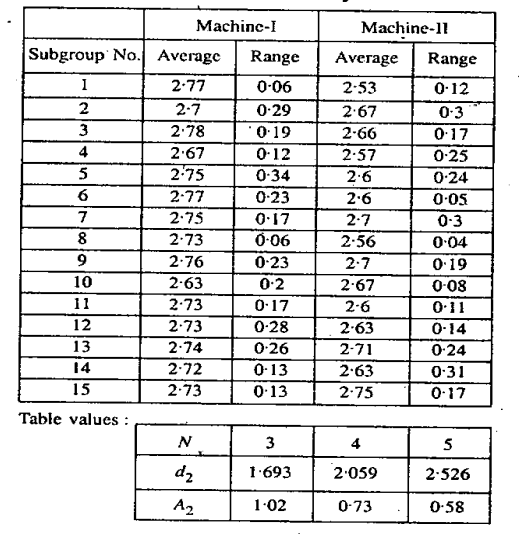
\includegraphics[]{IS/QC/4c2010.PNG}
    \caption{2010 - 4.(b)}
\end{figure}

